\documentclass[main.tex]{subfiles}

\begin{document}

  \section{Examples and Timings}\label{sec:examples_timings}

  \subsection{Timings}

  For testing purposes we consider two families of curves :
  \begin{itemize}
      \item reverse exponential series
          \begin{equation}
              \mathcal{E}_{m,n} : y^m = \sum_{k=0}^n\frac{x^{n-k}}{k!}
          \end{equation}
      \item reverse Bernoulli polynomials
          \begin{equation}
              \mathcal{B}_{m,n} : y^m = x^nB_n(\frac1x) = \sum_{k=0}^n\binom nkb_{k}x^k
          \end{equation}
  \end{itemize}

  The branch points of these two families present interesting patterns which can be considered as
  bad cases from a numerical integration perspective.
  \begin{figure}[H]
      \begin{center}
          \subfloat[degree 7]{ \includegraphics[width=.5\linewidth,page=3]{images/roots_exp.pdf} }
          \subfloat[degree 30]{ \includegraphics[width=.5\linewidth,page=4]{images/roots_exp.pdf} }
      \end{center}
      \caption{roots of reverse exponential polynomials.}
  \label{fig:roots_exp}
  \end{figure}

  \begin{figure}[H]
      \begin{center}
          \subfloat[degree 8]{ \includegraphics[width=.5\linewidth,page=3]{images/roots_bern.pdf} }
          \subfloat[degree 30]{ \includegraphics[width=.5\linewidth,page=4]{images/roots_bern.pdf} }
      \end{center}
      \caption{roots of reverse Bernoulli polynomials.}
  \label{fig:roots_bern}
  \end{figure}

  In the case of hyperelliptic curves, we compare our timings with the existing Magma code.
      \begin{center}
          \begin{table}[h!]
      \begin{tabular}{lllrrrrr}
          \toprule
          & & bits & 128 & 512 & 2000 & 4000 & 10000 \\
          curve & genus & digits & 38 & 154 & 600 & 1200 & 3000 \\
          \midrule
          $\mathcal{B}_{2,8}$ & 3
          & Arb   & 3e-3 & 7.9e-3 & 9.4e-2 & & 4.21            \\
          & & Magma (old) & 0.76 & 1.28 & 21.15 & 1190 & >1 month \\
          \midrule
          $\mathcal{B}_{2,30}$ & 15
          & Arb & 3.4e-2 & 1.5e-1 & 2.21 & & 92.1 \\
          & & Magma (old) & 8.070 & 15.260 & 283 & \\
          \bottomrule
      \end{tabular}
      \caption{timings in seconds for hyperelliptic curves.}
  \end{table}
      \end{center}

 
\biblio
\end{document}
